\documentclass[aasms,11pt, longbibliography]{article}
\usepackage{natbib}
\setlength{\bibsep}{0pt plus 0.3ex}
\usepackage[margin=1in]{geometry}
\usepackage{sectsty}
\usepackage{graphicx}
\usepackage{hyperref}
\usepackage{epstopdf}
\usepackage{anyfontsize}
\usepackage{wrapfig}
\usepackage[skip=2pt,font=small]{caption}
\captionsetup{width=\textwidth}
\usepackage{amssymb, amsmath, amsfonts, xcolor}
\hypersetup{
    colorlinks,
    linkcolor={red!50!black},
    citecolor={blue!80!black},
    urlcolor={blue!80!black}
}


\sectionfont{\normalsize}
\subsectionfont{\small}


%\citestyle{aa}
\newcommand{\aj}{The Astronomical Journal}
\newcommand{\apj}{The Astrophysical Journal}
\newcommand{\apjl}{The Astrophysical Journal Letters}
\newcommand{\apjs}{The Astrophysical Journal Supplemental Series}
\newcommand{\aap}{Astronomy \& Astrophysics}
\newcommand{\aaps}{Astronomy \& Astrophysics Supplemental Series}
\newcommand{\mnras}{Monthly Notices of the Royal Astronomical Society}
\newcommand{\baas}{Bulletin of the American Astronomical Society}
\newcommand{\zap}{Zeitschrift für Astrophysik}
\newcommand{\sol}{\ensuremath{\odot}}
\newcommand{\RB}{Rayleigh-B\'{e}nard }
\newcommand{\grad}{\ensuremath{\nabla}}

\usepackage{fancyhdr}
\pagestyle{fancy}
\fancyhf{} % sets both header and footer to nothing
\renewcommand{\headrulewidth}{0pt}
\renewcommand{\footrulewidth}{0pt}
\rfoot{\footnotesize{Evan H. Anders NSF AAPF 2019}}
\lfoot{\footnotesize{\leftmark}}
%\lfoot{\footnotesize{\leftmark}}%\thesection: \sectiontitle}}
\cfoot{\footnotesize{\thepage}}

\makeatletter
\renewcommand{\sectionmark}[1]{%
  \markboth{\ifnum \c@secnumdepth>\z@
      \thesection: \hskip 1em\relax
    \fi #1}{}}
\makeatother

\usepackage{titlesec}
%\titleformat{\abstract}[runin]{\normalfont\normalsize\bfseries}{\theabstract}{1em}{}
\titleformat{\section}[hang]{\normalfont\fontsize{14pt}{17pt}\selectfont\bfseries}{\thesection}{1em}{}
\titleformat{\subsection}[runin]{\normalfont\fontsize{12.5pt}{14pt}\selectfont\bfseries}{\thesubsection}{1em}{}
\titleformat{\subsubsection}[runin]{\normalfont\normalsize\bfseries}{\thesubsubsection}{1em}{}

\renewenvironment{abstract}
{
\noindent \par{\bfseries \abstractname.}}
{\medskip\noindent 
}





\begin{document}
\begin{center}
   \Large\textbf{Convective Conundrums in the Asteroseismic Age: }\\
   \Large\textbf{The interplay of rotation and magnetism in stellar convection  }\\
   \vspace{0.2cm}
   \large{Evan H. Anders}\\
   \vspace{0.2cm}
\end{center}

\vspace{-0.4cm}

\begin{abstract}
The past two decades have seen an impressive rise in our understanding of the interior structure of the Sun and countless other stars through helioseismic and asteroseismic techniques.
These observations often rely on inversions which are informed by simple models of stellar convection which do not include the important effects of magnetism and rotation.
Furthermore, these helioseismic observations of the Sun have called into question even our most fundamental understanding of stellar convection -- a problem widely referred to as the Solar Convective Conundrum.
Recent literature has suggested that complicating effects, such as rotation, may be the crucial pieces missing in our understanding.
During my postdoctoral studies, I propose to study how rotation and magnetism affect the dynamics of stellar convection from the smallest to the largest scales.
I will conduct detailed studies of individual stellar downflows and mesoscale studies of convective interactions at the radiative-convective interface.
I will further develop community tools to decrease the computational cost of global simulations of stellar convection, enabling improved stellar models and synthetic observables.
\end{abstract}

\vspace{-0.6cm}

\section{Motivation}
\sectionmark{Motivation}
\vspace{-6pt}

\subsection{Asteroseismology}
\label{sct:asteroseismology}
The advent of asteroseismic science has closely paralleled that of exoplanetary science.
The early small samples of stellar pulsations obtained by ground-based observatories \citep[e.g.,][and others]{kjeldsen&frandsen1991, bouchy&carrier2001, bedding&all2001} have given way to datasets of more than $10^4$ stars \citep[e.g.,][]{yu&all2018, santos&all2019b} in the age of CoRoT, Kepler, and K2 data.
With another 20,000 asteroseismically-interesting targets in the TESS satellite's two-year nominal mission \citep{schofield&all2019} and more interesting data from the future WFIRST and PLATO missions, it is expected that by 2030 we should have observations of $10^7$ pulsating red giants and $10^5$ dwarfs and subgiants in hand  \citep{huber&all2019}.
In addition to learning about the nature of stars aside from our Sun, asteroseismology enables us to fairly accurately determine the age of stars, thus enabling galactic archaeology, in addition to enabling us to determine the mass and radius of stars with solar-like pulsations, thus enabling the measurement of exoplanetary radii from the transit method.
Asteroseismic measurements generally rely on stellar structure models, and these models have some known deficiencies \citep{buldgen2019}, in particular their handling of complex phenomena like convection, rotation, and magnetism.
With the exponential rise in asteroseismic targets, and the projected continuation of this rise, it is crucial that the we continue to invest in the theory informing these stellar models and measurements.

The state-of-the-art method for obtaining stellar strucuture data is the use of one-dimensional models of stellar interiors from codes like MESA \citep{paxton&all2011}.
The coupling of MESA models and the GYRE code \citep{townsend&teitler2013} has enabled efficient identification of pulsational modes in a wide variety of stars.
Unfortunately, MESA models necessarily depend on one-dimensional parameterizations of convection and often employ the decades-old mixing length theory \citep[MLT,][]{bohm-vitense1958}.
MLT does an adequate job of describing convection within stars, but there are some well-known instances in which it regularly fails.
For example, 1D stellar models do not correctly produce the surface layers of stars with convective envelopes, but recent work suggests they fare better when coupled with three-dimensional surface simulations \citep{jorgensen&weiss2019}.
Furthermore, these one-dimensional models assume spherical symmetry and generally neglect the effects of rotation and magnetism.
The numerous observations of flare stars and recent asteroseismic observations which have detected magnetic field-induced frequency shifts \citep{santos&all2018} suggest that magnetism should not be neglected, and recent work shows that the specific configuration of the magnetic field impacts asteroseismic measurements \citep{thomas&all2019}.
Furthermore, it is well known that the sun exhibits differential rotation characterized by latitudinal variations in its rotational profile in the solar convection zone \citep{thompson&all1996, schou&all1998}, and differential rotation has now been observed in stars beyond the Sun \citep{benomar&all2018}.
These observations all suggest that a 1-dimensional parameterization of convection, and a neglection of complicating effects, cannot sufficiently capture the complexities of stars.
In order to properly and fully utilize the large stores of incoming asteroseismic data, we must improve the models on which asteroseismic inversions rely.

\subsection{The Solar Convective Conundrum}
\label{sct:convective_conundrum}
The Sun is our closest star, and it is a magnetically active star.
The collection of phenomena generally referred to as solar activity, including flares and coronal mass ejections, pose a threat to our increasingly technological society.
These phenomena can wipe out power grids and harm satellites and astronauts.
Predictive power of solar phenomena has been a decades-long research goal, but will be out of reach until we have a detailed understanding of the dynamo that drives solar activity.
This dynamo is seated in the turbulent convective plasma motions of the Sun, and recent observations have called into question even our most fundamental understanding of solar convection.

Helioseismic observations by \citet{hanasoge&all2012} place an upper limit on solar convective velocity magnitudes nearly two orders of magnitude lower than those predicted by simulations or MLT.
Other helioseismic measurements using different techniques claim detections of velocity magnitudes more in line with what is expected from theory \citep{greer&all2015}, but observe an unexpected decrease in powers at large scales compared to simulations.
Even observations of convective motions at the solar surface \citep{hathaway&all2015} do not observe these anticipated, large-scale motions.
Put simply, we do not see the theorized, large-scale ``giant cells'' which would be observational manifestations of buoyant motions driven deep in the solar convection zone.
This lack of giant cells consitutes part of the Solar Convective Conundrum, and two primary hypothesis which aim to explain their absence are the ``Entropy Rain'' hypothesis and a suggestion that the solar convective interior is rotationally constrained.

The entropy rain hypothesis, first suggested by \citet{spruit1997}, suggests that downflows alone carry the solar luminosity through the solar convection zone, and has been preliminarily incorporated into a modified mixing length theory by \citet{brandenburg2016}.
Some simple simulations of \citet{kapyla&all2017} suggest that indeeed downflows may be more important than upflows in determining convective properties in stellar envelope convection.
I conducted some recent theoretical work which suggests that such a mechanism could plausibly carry the solar luminosity in the deep solar convection zone \citep{andersLB2019}.
However, most or all of the work surrounding the entropy rain hypothesis neglects magnetism and rotation.
It is unclear how these complicating effects interact with fast, small downflows like entropy rain, and it is unclear how these raindrops would alter the rotational or magnetic structure of the Sun.

Outside of the entropy rain picture, it has also been suggested that the effects of rotation alone may be sufficient to explain the solar convective conundrum.
Simulations by \citet{featherstone&hindman2016} show that as convective flows become more rotationally constrained, the spherical harmonic degree of maximum velocity power of the convection increases.
However, simulations which nominally rotate at the solar rate show \emph{anti-solar} differential rotation \citep{gastine&all2014}, and simulations at very low rossby number exhibit either differential rotation that is too-cylindrical or more reminiscent of Jupiter than the Sun \citep{brun&all2017}.
Global simulations which both suppress giant cells and correctly produce the solar differential rotation profile have not been achieved.

\subsection{Modern convective simulations}
\label{sct:modern_simulations}
Early simulations in stellar-like convection \citep{graham1975, hurlburt&all1984, cattaneo&all1991, brummell&all1996, brummell&all1998} often sought to understand the nature of convection in toy models.
Simple geometries (Cartesian) were employed, and the nature of convection in the presence of one or more complicating effects (namely, stratification, rotation, magnetism, etc.) were explored.
As computational resources became more plentiful, these experiments gave way to simulations which aim to reproduce solar or stellar convection.
Small scale Cartesian domains of magnetohydrodynamic convection coupled with radiative transfer have produced results which look strikingly like solar surface convection and sunspots \citep{stein&nordlund1998, rempel&all2009, stein&nordlund2012, rempel2014}.
Large scale, ``global'' simulations of spherical rotating magnetoconvection have recreated cycling dynamos and differential rotation profiles \citep{brown&all2010, brown&all2011, guerrero&all2016, brun&all2017, strugarek&all2018}.
In addition to visually resembling features of solar convection, these modern simulations are being treated as observations.
For example, the simulations of \citet{rempel2014} have been treated extensively as high-resolution observations of solar convection\citep[see e.g.,][and others]{vankooten&cranmer2017, shchukina&trujillo2019} due to the precise knowledge of thermodynamic quantities as a function of depth, which cannot be simply obtained in true observations.
We are furthermore entering an age in which the wave spectrum in the outer layers of stellar simulations are being compared to those expected in asteroseismic theory \citep{edelmann&all2019}.

In the context of the coming asteroseismic observations, and in particular in the soon-arriving first light of the NSF's Daniel K. Inouye Solar Telescope (DKIST), having high-resolution synthetic observables on hand is extremely useful for calibration and scientific purposes.
However, in light of the convective conundrum, it is critical that we, as a community of modellers, take a step back and aim to understand the fundamental processes underlying stellar convection to ensure that our synthetic observables model fluid motions in the proper regime of stellar convection.
Small scale simulations where vast areas of parameter space can be explored like the earliest simulations have become rare \citep{wood&brummell2012, wood&brummell2018}.
The vast computational resources now available allow for extensive studies of these simplified systems, yet the highly laminar results of the simulations of two or more decades ago are still the state-of-the-art.
In our modern studies of simulations, simplified models \citep{brummell&all1998} should work hand-in-hand with complex local models \citep{rempel2014} and global models \citep{strugarek&all2018} to paint the fullest picture of stellar convection.
Through understanding convective dynamics at the smallest scales and using that understanding to influence our realistic models at the largest scales, we can move forward with confidence in coupling simulations and theory with observations.

\section{Intellectual Merit: Rotating magnetoconvection across all scales}
\sectionmark{Intellectual Merit}
\vspace{-6pt}

\label{sct:intellectual_merit}

Over the course of my postdoctoral studies, I will take advantage of the flexibility of the Dedalus pseudospectral framework \citep{burns&all2019}, which I have become proficient at using during my graduate career, to study numerical simulations at three different scales.
In task A (section \ref{sct:taskA}), I will study simulations of discrete events, or thermals \citep[as in ][]{andersLB2019}, which model stellar convective downflows and can achieve high levels of turbulence.
In task B (section \ref{sct:taskB}), I will study simulations of mesoscale convection \citep[as in ][]{anders&brown2017} to gain an understanding of how these effects behave in the presence of the convective-radiative interface.
In task C (section \ref{sct:taskC}), I will study simulations of global stellar convection, developing and using new tools within the Dedalus framework to study the importance of rotation and magnetism over relaxational timescales.
Each task is expected to take one full year of my three-year postdoctoral fellowship.
Over the course of these three tasks, I will aim to understand two fundamental questions.
First, how do convective motions transport angular momentum and magnetic fields, and does resolving turbulent flows change this answer?
Second, how do rotation and magnetism feed back upon convective dynamics?

\subsection{Task A: Dynamics of individual downflows}
\label{sct:taskA}
\begin{wrapfigure}{l}{0.4\textwidth}
	\begin{center}
	\vspace{-10pt}
    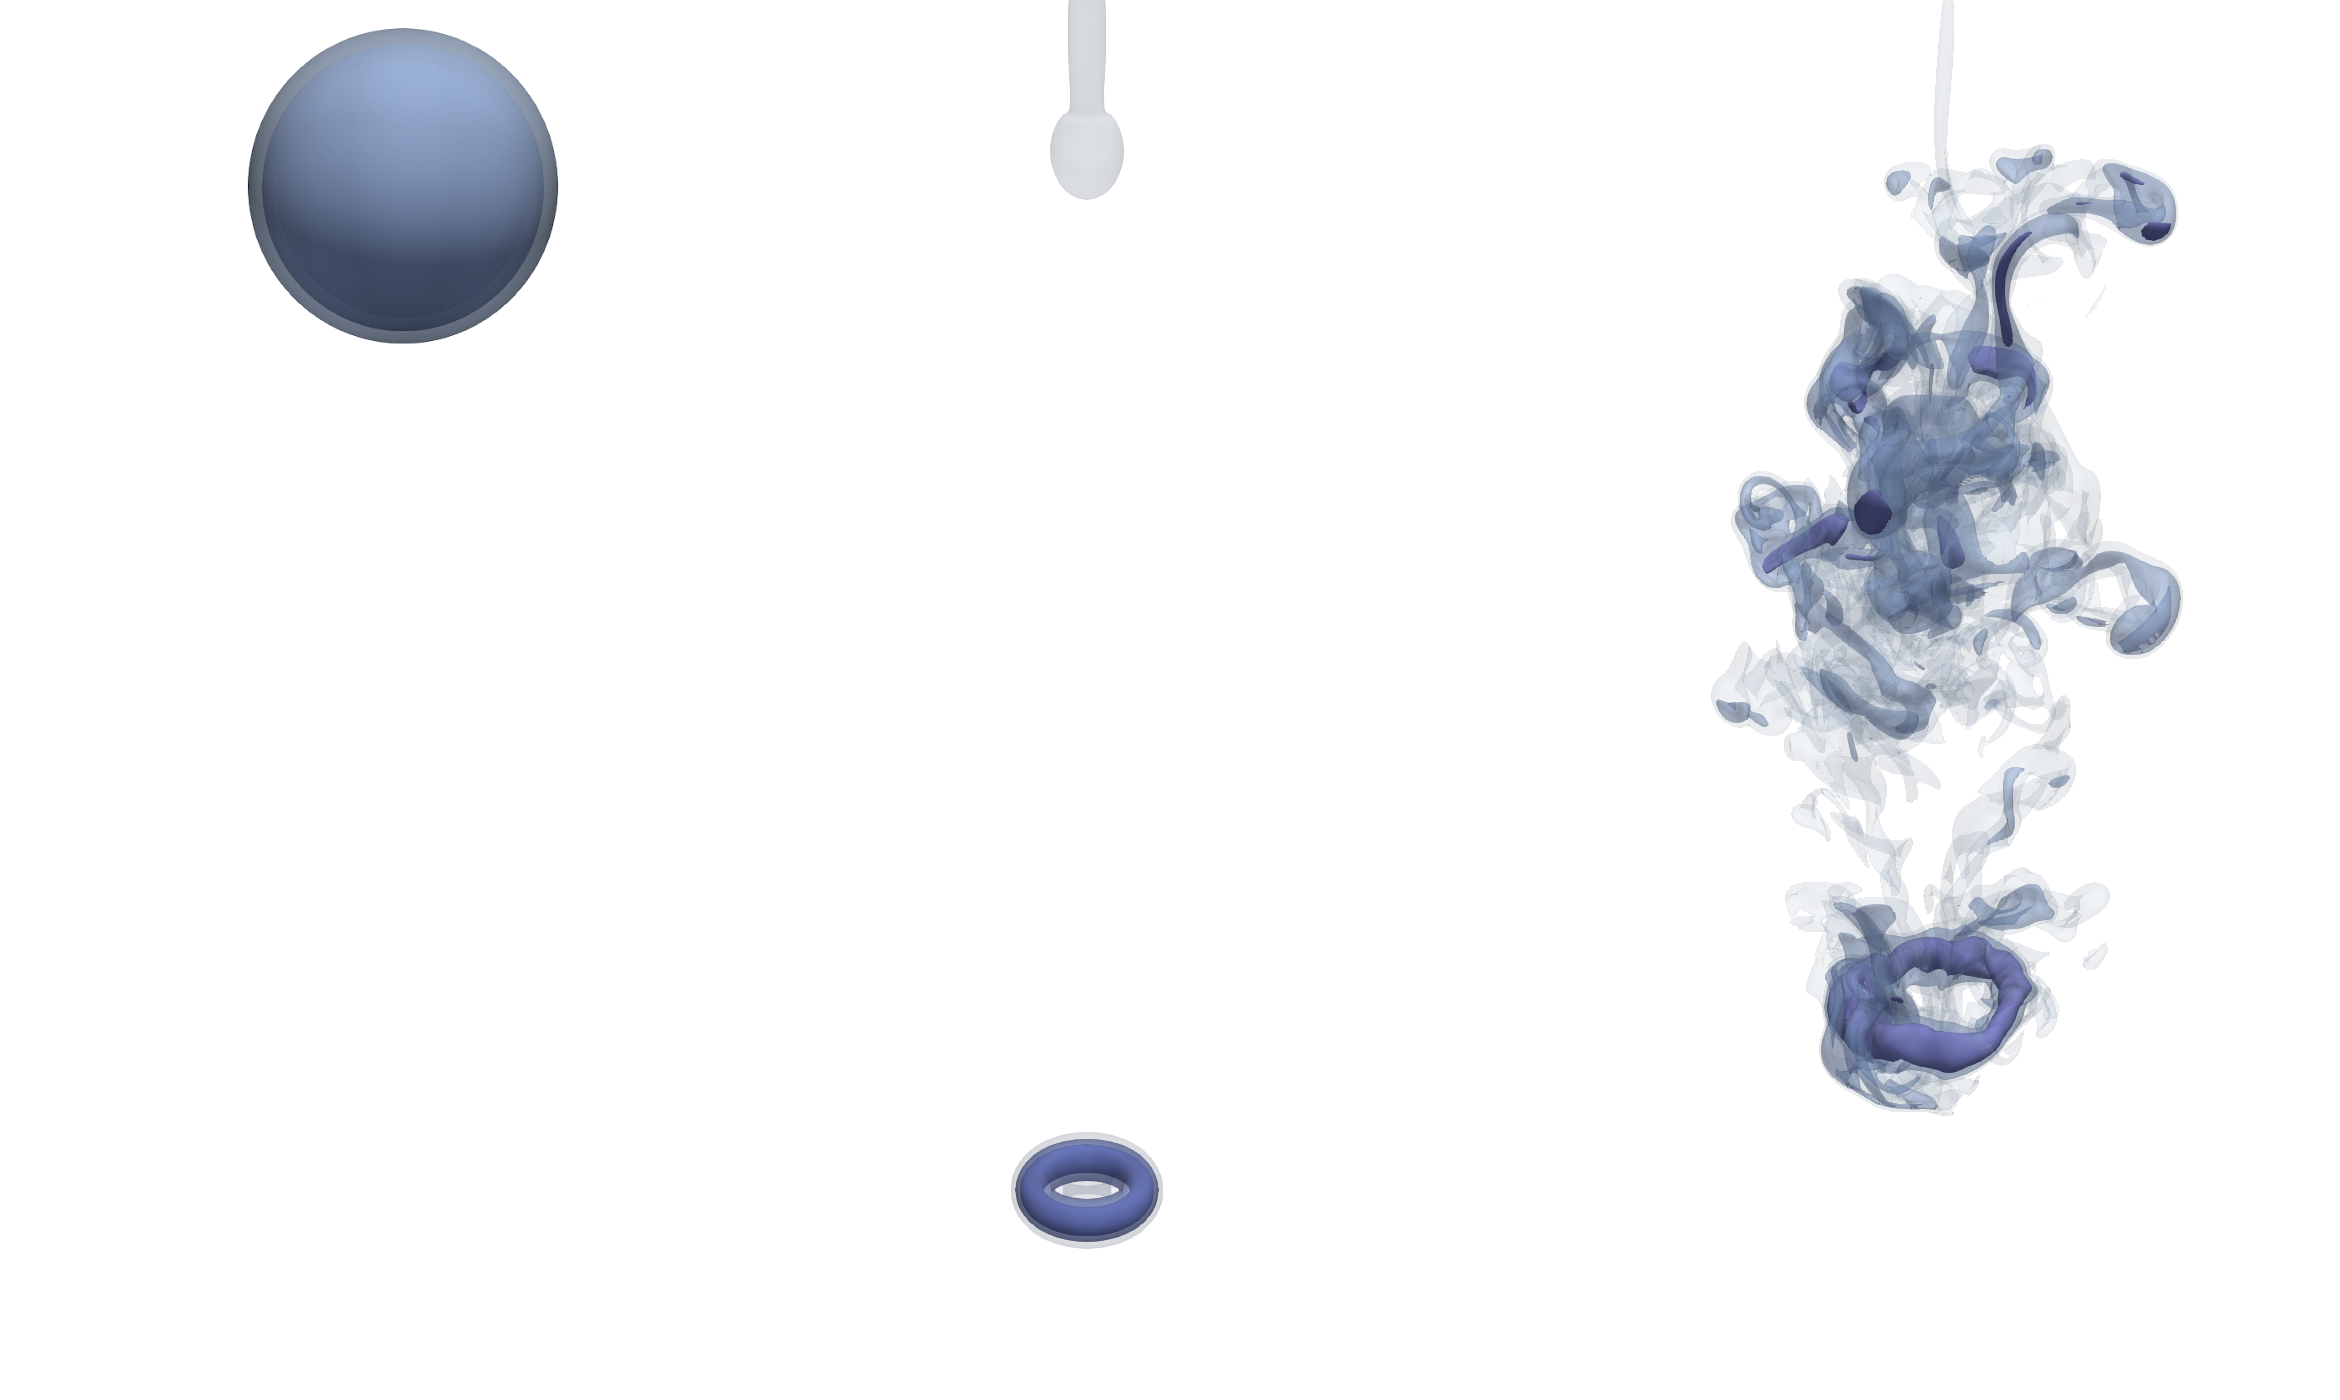
\includegraphics[width=0.38\textwidth]{./figs/thermals_comparison.png}
	\vspace{-15pt}
	\end{center}
    \caption{
	3D visualizations of the entropic signature of evolved thermals in the laminar (left) and turbulent (right) regimes.
	\label{fig:thermals_comparison} }
\end{wrapfigure}

In the envelopes of lower main sequence stars, convection occurs in the presence of extreme stratification.
Stratified convection is characterized by powerful, localized downflows, and broad, slow upflows.
Recent theory and observations (section \ref{sct:convective_conundrum}) suggest that downflows may be the predominant mechanism for transporting stellar luminosity in these convective zones.
Furthermore, \citet{tobias&all1998} showed that downflows in convection can effectively pump magnetic fields downwards in certain regimes.
These results suggest that downflows in stratified convection deserve careful study.

Downflows may turbulently break up into distinct pieces as they fall and these pieces can be modeled as thermals.
Thermals are regions of cold fluid which accelerate due to buoyancy forces and shape themselves into vortex rings; evolved thermals are visualized in Fig. \ref{fig:thermals_comparison}.
Thermals are observed and studied in the Earth's atmosphere and well understood in the Boussinesq limit.
Recently, I studied thermals as a model for solar convection and came to understand the effects of stratification on the propagation of thermals \citep{andersLB2019}.
%I developed a theory for the effects of stratification and conducted high resolution simulations of thermals which verified that theory.
%I now propose to extend that stratified work to further include the effects of rotation and magnetism.

Thermals provide an excellent model of stellar downflows because they are relatively easy to model analytically and to simulate.
Hydrodynamic thermals in stratified domains have a solution which is essentially fully specified by: (a) the stratification that they feel and (b) whether they are laminar or turbulent.
Thanks to my work in \citet{andersLB2019}, the influence of stratification on thermals is now understood.
During my postdoctoral studies, I will study thermals in a fixed high-stratification regime and gain a theoretical and experimental understanding of the effects of magnetism and rotation on thermal evolution.
In a purely hydrodynamical context, \citet{lecoanet&jeevanjee2019} showed that turbulence does not appreciably change the evolution of thermals.
However, turbulence creates smaller scale structures in the propagating thermals which may be important in the context of rotation or magnetism.

\subsubsection{Task A.1: Rotational filtering of downflows}
\label{sct:taskA1}
In order to study the effects of rotation, I will study thermals in simple Cartesian domains.
These plane-parallel atmospheres exist at a fixed latitude and experiencing Coriolis forces from a global rotation rate.
%This complication will allow me to study the effects of rotation as a function of latitude, and in regimes where rotation is more and less important.
I propose to study downflows at the equator, poles, and mid-latitudes.
At each of these latitudes, I will study flows which experience varying degrees of rotational constraint.
I will initially study laminar thermals to understand parameter space, but will later examine select turbulent simulations in all regimes which exhibit distinctly different behavior.
The primary goal of these studies will be to determine at which latitudes, and at which degrees of rotational constraint do Coriolis forces prevent thermals from transiting the convection zone.
These results will help determine which stellar regimes could benefit from the implementation of a nonlocal mixing length theory \citep[as in][]{brandenburg2016}.

\subsubsection{Task A.2: Transport of magnetism by downflows}
\label{sct:taskA2}
I will secondarily study thermals in the presence of magnetism but absence of rotation.
The inclusion of magnetism requires a choice of initial magnetic field setup, and I will study both cases in which there is a uniform background field and where there is a thin horizontal sheet of magnetism for the thermal to pass through \citep[as in][]{tobias&all1998}.
I will vary the orientation of the initial magnetic fields and the degree of influence of magnetism on the flows, in a manner analagous to the rotational simulations in Task A.1.
These simulations will help determine how the role downflows play in the transport and generation of magnetic fields in the solar dynamo.
This work will further constrain regimes in which magnetism prevents downflows from transiting convection zones, analagously to task A.1. 

\subsection{Task B: Mesoscale interactions at the tachocline}
\label{sct:taskB}
\begin{figure*}[t!]
    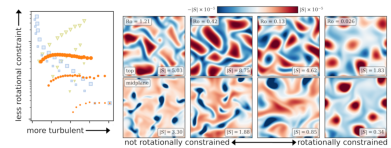
\includegraphics[width=\textwidth]{./figs/rossby_plot.png}
    \caption{(left, Fig 1b of \citet{anders&all2019}) The Rossby number, Ro, is difficult to predict as a function of the Rayleigh number, Ra, in rotating convection.
	Along traditional ``convective Rossby number'' (green) paths through parameter space, Ro increases as a function of Ra, and along constant supercriticality paths (blue) it decreases.
	Walking along paths along the newly discovered ``predictive Rossby number'' (orange) seems to hold the value of Ro, and thus the degree of rotational constraint, constant.
	(right eight panels, Fig. 2 of \citet{anders&all2019}) As you decrease the Rossby number (from left to right), traditional granular convective patterns give way to quasi-two-dimensional vortical columns of convection with very little difference between the top of the atmosphere and the atmospheric midplane (top row vs. bottom row).
	It is clear to see that changing the Rossby number strongly affects convective dynamics and therefore choosing a value of Ro that reflects the astrophysical object of interest being studied (e.g., the Sun) is crucial.
	\label{fig:rossby_plot} }
\end{figure*}

In solar-like stars, the strongly stratified convective zone overlies a stable interior radiative zone.
In the Sun, the region which separates these two zones is called the tachocline, and is characterized by both a transition from instability to stability and also a strong shear in the angular velocity as the differential rotation of the convective zone gives way to the uniformly rotating solar interior.
I will refer to the radiative-convective boundary as a ``tachocline,'' and here I propose studying convective interactions at such an interface in the absence of angular velocity shear. 
Recent results suggest that convecting regions which reside above stable layers may depend primarily on downflows to transport energy fluxes \citep{kapyla&all2017}.
This begs the question: how does increased stratification in the convective zone, and the more intense downflows that accompany it, affect interactions at the tachocline?
A further piece of disagreement in current theory centers around the depth to which convective motions penetrate below the tachocline.
The magnitude of deep convective velocities and the strength of stability of the radiative zone should determine this, but deep velocity magnitudes are poorly constrained.
As a result, I propose studying how the stiffness of this interface, which characterizes whether convective motions feel a soft or hard tachocline \citep{couston&all2017}, affects the transport of angular momentum and magnetic fields into the radiative zone.

Flow balances in evolved convective dynamics are often difficult to predict from input parameters.
However, during my graduate career, I indentified and verified mechanisms for controlling the evolved Mach number \citep{anders&brown2017} and degree of rotational constraint \citep[][and Fig. \ref{fig:rossby_plot}]{anders&all2019} in mesoscale convection simulations.
The first step of Task B will use similar techniques in order to determine how to set the degree of magnetic constraint in these magnetorotational simulations.
Using that knowledge and the knowledge of task A, I will study the importance of stratifiation and stiffness of the tachocline in regimes in rotating magnetoconvection which are interesting in the stellar context.

\subsubsection{Task B.1: Controlling the importance of magnetism}
\label{sct:taskB1}
In simple models of convection, it is straightforward to control the degree of turbulence of the evolved state.
Once complicating physics are included, such as rotation and magnetism, determining the nature of evolved convective flows becomes increasingly difficult.
Interactions between boundary conditions, boundary layers, and bulk dynamics are complex and complex paths must be walked through parameter space in order to remain in specified dynamical regimes.
In \citet{anders&all2019}, I determined an appropriate path through parameter space for holding the degree of rotational constraint constant.
In this subtask, I will study nonrotational magnetoconvection and determine how to control the importance of magnetic interactions on convective flows.

\subsubsection{Task B.2: Downflow interactions at a stiff tachocline}
\label{sct:taskB2}
A strongly stratified convection zone should be characterized by intense downflows, and in this subtask I will determine how these downflows interact with different types of tachocline.
I will study very stiff tachoclines, which act similar to hard boundaries, and very soft tachoclines which convective motions can easily pass through.
\citet{tobias&all1998} showed that convective motions can effectively pump magnetic fields across soft tachoclines in certain parameter regimes.
Here I will extend that work  to determine if magnetic fields and angular momentum are capable of being pumped into stiff tachoclines by convective motions.
These simulations will be guided by the work done in Task A, and will be studied at latitudinal, rotational, and magnetic regimes in which downflows should be able to persist through the solar convective zone.
It is widely believed that the tachocline is a critical piece of the solar dynamo, but if convective motions are not able to pump magnetic fields into a stiff tachocline, then a different mechanism must be responsible for generating new magnetic fields.
Furthermore, a stiff tachocline could potentially insulate the solar radiative interior from convectively-driven angular momentum transport, which could help explain the uniformly rotating solar interior.
In short, these suites of simulations will ask whether our picture of the solar dynamo should change in the presence of a stiff tachocline.

\subsection{Task C: Global studies in relaxed atmospheres}
\label{sct:taskC}
The capstone project of my postdoctoral studies will study convection at the largest scales: global spherical simulations of rotating magnetoconvection.
The tools to perform these simulations in Dedalus already exist \citep{lecoanet&all2018} and have been tested.
One major barrier to performing global simulations is that they are costly, and some of these costs are unavoidable: highly resolved, moderately turbulent simulations necessarily take small timesteps, and therefore results come slowly.
However, some of the expense of these simulations is often time wasted waiting for the atmospheric structure and mean flows to converge to an equilibrium state.
For example, the thermal structure of the Sun is thought to evolve over its Kelvin-Helmholtz timescale of $10^7$ years, which is significantly longer than its convective overturn time of five minutes at the solar surface, although still much shorter than its main sequence lifetime.
As simulations approach the parameter regime of stars, relaxation and dynamical timescales become extremely disparate, and in general numericists must choose between having state-of-the-art turbulence or converged, statistically equilibrium dynamics -- but not both.
During this third task, I will develop, test, and utilize a community tool which effectively establishes mean flows and evolves atmospheric structures by taking much larger timesteps than those of convection.
By doing so, I will enable global dynamo simulations which are both relaxed and exhibiting state-of-the-art turbulence.

During my graduate career, I studied a mechanism for accelerating the long thermal relaxation timescale in convective systems \citep{anders&all2018}.
In this work, we discovered that a tool like the one I am proposing here can be feasibly implemented and tested for accuracy, albeit we previously studied this in a very simple system.
While studying moderately turbulent flows, we found that our tool reached a relaxed state using an order of magnitude fewer computational resources than when waiting for a standard thermal relaxation timescale.
These speedups make achieving thermal relaxation in state-of-the-art simulations feasible.

\subsubsection{Task C.1: Accelerated evolution of global simulations}
\label{sct:taskC1}
During my postdoctoral studies, I will extend my accelerated evolution method to the evolution of thermodynamic and angular momentum profiles in global simulations.
The development of this extension will be grounded in understandings gained in tasks A and B.
In particular, task A will inform which terms in the equations importantly adjust the mean field in certain regimes, and task B will inform how to implement this technique near tachocline-like interfaces.
As I did in \citet{anders&all2018}, I will verify that this method produces the same results as a long relaxation in modest parameter regimes to build trust in the method.
Once developed, this Dedalus module will be made publicly available.

\subsubsection{Task C.2: Relaxed simulations of the solar dynamo}
\label{sct:taskC2}
I will study simulations of the interior solar convection zone in regimes where flows feel the effects of both rotation and magnetism, using the knowledge from task B.1 to determine how to set up such simulations.
Using the tool developed in task C.1, I will accelerate the evolution of these simulations.
I am predominantly interested in the relaxed differential rotation profiles that appear as a function of rotational constraint, and how these differential rotation profiles affect the time evolution of the magnetic dynamo.
In most modern dynamo simulations, the evolution of magnetic fields are measured during the relaxation process, and it is possible that the time-dependent dynamo behavior of the simulation is strongly influenced by the underlying evolution of the mean state.

While these simulations will be largely targeted in the solar context, the accelerated evolution tools which will be developed and tested here could have great benefits for asteroseismic research.
Recently, \citet{jorgensen&weiss2019} coupled three-dimensional, global simulations with 1-dimensional stellar structure tools in order to more accurately produce stellar structure profiles to great success.
The fast equilibration of angular momentum and thermal profiles described here is essentially equivalent to taking timesteps which superstep the convective motions, similar to those taken in any one-dimensional stellar structure model.
Put simply, these accelerated evolution techniques would be a first step to enabling a generalized coupling of 1-dimensional stellar structure codes with realistic statistics from converged global convection.
Future asteroseismic inversions will then benefit from stellar structure models which are influenced by three-dimensional convection including complicating effects like magnetism and rotation.

\subsection{Computational Feasibility}
\label{sct:feasibility}
Tasks A-C are arranged logically from smallest to largest scales, and also from least to most computationally expensive.
Based on the work in \citet{anders&brown2017, anders&all2018, anders&all2019, andersLB2019}, Dedalus takes $\mathcal{O}(10^3)$ cpu-sec per iteration for a run with a grid resolution of 384$^3$ on a system comparable to NASA Pleiades.
Task A runs of thermals will take $\mathcal{O}(10^4)$ iterations each, while turbulent runs in tasks B and C will take $\mathcal{O}(10^6)$ iterations each.
Laminar thermal simulations thus cost roughly 5000 cpu-hours each, while turbulent thermals cost roughly $10^5$ cpu-hours each.
State-of-the-art simulations in tasks B and C will cost roughly $10^6$ cpu-hours each.
The projects described here total 5-10 million cpu-hours per year in tasks B and C, with less (2-3 million cpu-hours) in the first year while thermals are being studied.

The computational cost of task A should be feasible to obtain on Northwestern's 11,800-core Quest supercomputer.
In order to increase my access to computational resources and to allow for larger scale runs in tasks B and C, I will leverage my AAPF fellowship and apply for time on NSF XSEDE resources such as Stampede2, Comet, or Bridges.


\section{Collaborative studies at CIERA}
\sectionmark{CIERA}
\vspace{-6pt}

\label{sct:ciera}
Northwestern university, and specifically the Center for Interdisciplinary Exploration and Research in Astrophysics (CIERA), is the perfect location for me to carry out the work proposed here.
Dr. Daniel Lecoanet, who will be my primary advisor and collaborator, is one of Dedalus' founders.
His expertise using Dedalus and his past work on thermals \citep{lecoanet&jeevanjee2019, tarshis&all2018}, convection \citep{lecoanet&quataert2013, lecoanet&all2014, couston&all2017}, rotating convection \citep{couston&all2019}, and global simulations \citep{lecoanet&all2018} make him excellently qualified to advise me on the projects proposed here.
Furthermore, I have already published a paper on thermals in close collaboration with Dr. Lecoanet \citep{andersLB2019}, so task A will serve as an excellent transition project into my postdoctoral studies on my arrival.
In addition to Dr. Lecoanet, Dr. Yoram Lithwick would be an excellent partner for collaboration due to his past work on rotating convection \citep{BDLithwick2014} and his continuing collaborations studying careful and numerical problems in fluid disks \citep{LDLithwick2019} and planetary systems \citep{hadden&lithwick2018}.
Despite working on disparate applications, I anticipate that the work proposed here will benefit from fruitful conversations with other members of the institute, such as Dr. Sasha Tchekhovskoy, whose background in general relativistic MHD simulations is extensive \citep[as in e.g.,][]{tchekhovskoy&bromberg2016}.

Furthermore, in addition to the focused educational and outreach projects described below in section \ref{sct:broader_impacts}, CIERA will provide me with numerous small scale opportunities to participate in public outreach.
CIERA's Astronomy on Tap program as well as its CIERA Astronomer Evenings provide bite-sized and accessible ways to interact with the public.
Dearborn Observatory's observation tours are very similar to the public open houses I helped host at CU Boulder's Sommers-Bausch observatory.
The state-of-the-art Adler planetarium also provides similar opportunities such as its \emph{`Scopes in the City} program or its Space Visualization Lab astronomy conversations.


\section{Broader Impacts: Supporting young career scientists as educators and individuals}
\sectionmark{Broader Impacts}
\vspace{-6pt}
\label{sct:broader_impacts}
During my time at CIERA I will implement two small programs which leverage existing programs and institutes at Northwesten and whose outcomes align with NSF broader impact goals.
The first program, described in section \ref{sct:inquiry_class} will improve STEM educator development at the university level while also increasing public engagement with science at the high school level.
The second program, described in section \ref{sct:mentoring} will help improve participation of women, persons with disabilities, and underrepresented minorities in STEM.

During my graduate career I participated twice in the University of California Santa Cruz's Institute for Scientist and Engineering Educators Professional Development Program (UCSC ISEE PDP), an NSF-funded program during which early career scientists spend roughly 100 hours learning the basics of teaching pedagogy while developing and teaching an authentic STEM inquiry activity.
I further spent three years as a graduate student administrator with the CU-STARs group (University of Colorado Science Technology and Astronomy RecruitS).
CU-STARs is a combined ``outreach'' and ``inreach'' program with the dual aims of increasing STEM engagement for students at underserved, rural schools across Colorado while decreasing attrition of underrepresented groups in CU Boulder's Astrophysical and Planetary Sciences department.
On top of these activities, I was a co-instructor of record for an introductory Python programming course two years ago, and my co-instructor and I completely redesigned the course curriculum before we taught the course.
These experiences have greatly informed the design of the programs presented below, and have provided me with the tools to succeed at implementing these programs.

\subsection{Developing early career scientists as teachers}
\label{sct:inquiry_class}
I propose to work collaboratively with the CIERA-based and NSF-funded \href{http://gk12.ciera.northwestern.edu/}{Reach for the Stars} program, a GK-12 program, to develop a one-quarter course for graduate students and senior undergraduate students which teaches the basics of teaching pedagogy and culminates in authentic teaching experiences in high school classrooms.
Many young scientists do not have an opportunity to learn about teaching pedagogy or to develop any part of a curriculum during their undergraduate or graduate preparation, and this course will provide this opportunity in a contained scope.
I will spend 10-15\% of my time during my first year as a postdoctoral researcher developing and establishing the infrastructure for this course, then I plan to teach the course in the winter quarter of 2022 and 2023.
Over the course of spring, summer, and fall, I will iterate and improve on my course materials based on student performance and feedback; during spring and summer of 2023 I will further ensure that the course materials are made available to Northwestern faculty before my fellowship ends.

Students will work in small groups to design a multi-day, authentic learning experience that is guided by a specific set of learning goals in a high school curriculum.
I will leverage connections with Reach for the Stars in order to partner with high school teachers who will both provide a venue for course students to teach in and who will set the learning goals around which the activities will be designed.
Reach for the Stars is a selective program which offers a small number of graduate students an opportunity to spend 10-15 hours per week in high school classrooms leading young students through authentic scientific inquiry experiences while teaching those students how to think computationally and use computational tools.
This class I am proposing here will complement Reach for the Stars by providing an opportunity for professional growth and impactful outreach to a larger number of students which is overall a smaller time commitment and less selective.

One guiding principle of proper course design is backwards design \citep{wiggins&mctighe1998}, which is \emph{logically} foward, but \emph{in practice} backwards from how many courses are designed.
In essence backward design states that you start with the learning outcomes you want your students to achieve, then you design careful assessments to determine whether or not those learning goals were met, and \emph{only then} do you design the course content.
Students who take this course will use the backwards design process to design their inquiry activities, and working under the constraints set by the high school curriculum will enforce this content.
In general, this course will cover four broad topics, each of which has been heavily influenced by the groundwork and structure of ISEE's PDP program:
\begin{enumerate}
\vspace{-9pt}
\item Students will learn backwards design, and apply those principles in the context of their activity.
Students will learn how to set clear learning goals which leave space for authentic inquiry while also ensuring their learners arrive at desired learning outcomes.
\vspace{-9pt}
\item Students will learn about different types of assessments (e.g., tests, worksheets, etc.), when these assessments are appropriate, how to create honest and fair rubrics, and how to align a rubric with an assessment.
\vspace{-9pt}
\item Students will learn about and discuss equity and inclusion in the context of course design, including reading published research regarding the effects that inequities have on student achievement, and incorporating elements of inclusive design into their activities with multiple pathways for success so that all learners can achieve the learning goals.
\vspace{-9pt}
\item students will teach in the high school classroom, and then will learn about and practice methods for iterating on course design in order to improve it for improved learning outcomes in the future.
\vspace{-9pt}
\end{enumerate}

This course will develop scientist educators by providing young career scientists with a foundation in teaching pedagogy, and will also give them an opportunity to try out some teaching practices in a fairly low-stakes setting.
Assessments throughout the course will grade students on their creation, analysis of, and reflection on their course design rather than on the specific teaching outcomes of their activity.
Furthermore, the culminating project for each group of students is by definition an outreach activity: the students will go into nearby high school classrooms, engage with young students about science, provide authentic and inclusive experiences in STEM, and in doing so increase STEM engagement in the nearby community.
These outreach activities will expose high school students to authentic STEM practices, such as creating hypotheses or designing and carrying out investigations.
These practices are often not explicitly taught, and this can make it difficult for scientists to communicate their processes.
Reach for the Stars' \href{https://avault.github.io/}{Vault} program does an excellent job of providing a space for students to participate in these practices.
While designing this course, I will collaborate with Reach for the Stars and utilize modern literature \citep[e.g.,][]{dasgupta&all2014} to ensure that students in my course understand struggles that students face in learning the practices of science so that their learners can engage with STEM in this meaningful way.

\subsection{Undergraduate and graduate peer mentorship}
\label{sct:mentoring}
I propose to work with the experts in Northwestern's \href{https://www.northwestern.edu/searle/index.html}{Searle Center for Advanced Teaching and Learning} to develop peer mentoring programs within STEM departments at Northwestern University.
The goal of this program will be to connect students with peers who are slightly more advanced in their careers.
For example, entering undergraduate mentees would connect with junior or senior undergraduates in the field; senior undergraduates mentees could connect with young graduate student mentors; young graduate student mentees could connect with senior graduate students; and senior graduate students could connect with postdoctoral researchers.
In general, we would aim to connect young scientists who are still at a close enough level of their career to fully understand the experiences of one another to give young students advice and provide them with a professional support network.

It is well known that the path to a career in the US STEM workforce is a leaky pipeline.
Data show that in particular, women and many minority groups pursue careers in STEM fields at a rate which is disproportionately low compared to the share of the total population that those groups constitute \citep{corbett&hill2015, nsf2019}, and they are therefore underrepresented in the STEM workforce.
While a great deal of focus is rightly placed on changing the career outlooks of these groups before the collegiate level, underrepresentation becomes increasingly more severe at the baccalaureate and post-baccalaureate levels.
Mentoring has long been known to play a significant role in increasing retention and helping new departmental members acclimate to the department climate \citep{hunt&michael1983}.
Establishing robust mentoring programs based on evidence and knowledge of the recent literature in mentorship \citep[as in e.g.,][]{crisp&all2009, crisp&all2017} can be one critical component of helping broaden participation of underrepresented and marginalized groups in the STEM workforce.

I will lay the groundwork for this program in the remaining 10-15\% of my education time in my first year at Northwestern and roll it out during the fall quarter of 2021.
My first year will be spent collaborating with the departments of Physics and Astronomy, Applied Math, and others in order to gain university buy-in at the faculty level to ensure that this program will continue to run after I leave.
I will also collaborate with the Searle Center and others to ensure that I establish proper training for mentors.
Furthermore, I will begin searching at the University level for sustainable \href{https://www.northwestern.edu/studentorgs/org-officers/funding/index.html}{funding} so that this organization can support the purchasing of coffee and snacks for mentor meetings in order to encourage increased participation.

\subsection{Personal career growth and development}
\label{sct:personal_growth}
My graduate career and the experiences within it have given me confidence that I enjoy teaching as much as research, and so my eventual career goal is to become a professor at the university level.
By developing the course proposed in section \ref{sct:inquiry_class}, I will get to continue to hone my own course design and teaching skills while also providing many early career scientists an opportunity to interact with teaching in a substantial way.
Through my outreach experience in CU STARs, I have an understanding of how to interact with high school programs and teachers, which will be necessary for the development of my course in section \ref{sct:inquiry_class}.
Furthermore, one of my many roles as a graduate student administrator in STARs was to mentor undergraduate students, and this experience has laid the groundwork for my desire to set up the mentoring program described in section \ref{sct:mentoring}.
I know that in addition to research duties, being a professor includes a great deal of teaching, departmental service, and collaboration with university institutions.
These proposed programs will help me to continue to develop as a teacher, as a negoatiator, and as an active contributor to a healthy departmental culture.

\section{Summary and Perspectives}
\vspace{-6pt}
Observations of pulsating stars are becoming plentiful, and asteroseismic processing of those observations requires models which depend upon simple studies of convection.
However, observations of the Sun have revealed that our parameterizations of convection do not adequately describe this complex process in the stellar and solar context.
Numerical simulations at all scales and all levels of complexity have been useful tools for building theory and understanding or reproducing observations.
Modern simulations often focus on overly complex systems, and here I propose simulations at both small and large scales which sequentially build upon and inform one another.

The simulations proposed are necssary and timely.
As continued observations pour into our databases from current and future missions, it is crucial that we do not allow the theoretical pieces of observational pipelines to be neglected.
Current convective models cannot explain the Convective Conundrum and the combined effects of downflows, rotation, and magnetism is unclear and has not been well explored.
Furthermore, at a time when simulations are increasingly being treated as obervations, the development of tools such as those in Task C which help ensure that convective models more accurately reflect the physics at work in stars is crucial.

The fundamental problems presented here are of broad scientific interest, but are specifically topics of NSF investigation, as evidenced by the NSF's support for the DKIST telescope which will soon come online.
The collaborative studies centered at CIERA will address the following key questions:
\begin{itemize}
\vspace{-9pt}
\item Is the Sun in a regime where entropy rain is its dominant convective process and in which rotation and magnetism do not prevent this mechanism from occuring?
\vspace{-9pt}
\item Is the stability of the tachocline important in driving the solar dynamo and the Sun's latitudinal differential rotation profile?
\vspace{-9pt}
\item What rotational regime is the Sun in, and what can we learn about dynamo evolution in that regime?
\vspace{-9pt}
\end{itemize}

As stated previously, the work designed as Task A will occupy my research time during my first year while I lay the groundwork for my mentorship program and course on teaching pedagogy.
Task B will occupy my time during my second year, while I launch my mentorship program, teach my class for the first time, and work to improve both of these programs.
I will cap off my time at CIERA with task C while I work to ensure that the programs and classes that I set up smoothly transition to new leadership when I leave so that future students can continue to benefit from these programs.


\newpage
\bibliographystyle{yahapj}
\bibliography{biblio}
\end{document}
